
\documentclass[10pt]{article}
\usepackage{graphicx}
\addtolength{\oddsidemargin}{-.875in}
	\addtolength{\evensidemargin}{-.875in}
	\addtolength{\textwidth}{1.75in}

	\addtolength{\topmargin}{-.875in}
	\addtolength{\textheight}{1.75in}
\renewcommand{\baselinestretch}{0.97}
\title{Assignment 1}
\author {Harshdeep Gupta, 2013MT60597\\Deepali Gupta, 2013MT60079}

\date{Due date: January 25, 2017, 11:55pm IST}

\begin{document}

\maketitle

\section{Answer 1}
\subsection{ER Diagram}
 \begin{center}
\includegraphics[width=16cm]{ER.png}{\\ER Diagram}
\end{center}
%%% Fill in your content here.
\begin{table}[h!]
  \centering
  \caption{Entities and Attributes}
  \label{tab:table1}
  \vspace{5mm}
 
  \begin{tabular}{|p{2cm}|p{10cm}|p{3cm}|}
    \hline
    Entity & Attributes & Keys\\
    \hline
    \hline
    Degree & ID, Name, Curriculum, Pricing, Admission, AboutTheProgram DisplayImage& ID\\
    \hline
    Specialization & ID, Name, Price, Description, DisplayImage & ID\\
    \hline
    Course & ID, Name, Topic, Price, Session, BasicInfo, Level, Language, DisplayImage, HowToPass, UserRatings, CourseReviews, AboutTheCourse, WhoIsThisCourseFor, Syllabus, CertificateOffering, Description & ID \\
    \hline
    Institution & Name, Region, Description, DisplayImage, Contact Details & Name, Region\\
    \hline
    User & ID, Name, Photo, Location, Gender, Birthday, AboutUser, Websites, Privacy, Purchases & ID\\
    \hline
    Instructor & UserID, Designation, Twitter Handle, Department, Description & UserID\\
    \hline
    Assignment & Index, Title, Deadline, ToPass, Weight, Grade, Questions & CourseID, Index\\
    \hline
%     Question & Index, Statement, Answer & CourseID, AssignIndex, Index\\
%     \hline
    Video & ID, Title, Transcript, Likes, Subtitles, Resources, Language & ID \\
    \hline
    Forum & ID, Topic, Guidelines, Description, No of threads, Last updated & ID\\
    \hline
    Thread & ID, UserID, Title, Post, Views, Likes, Last Posted, Content & ID\\
    \hline
    Comment & ID, UserID, Statement, Likes, PostedAt & ID\\
    \hline
    Reply & ID, UserID, Statement, Likes, PostedAt & ID\\
    \hline
    FAQ & ID, Index, Question, Answer & ID\\
    \hline
    Resource & Index, Type, Title, Content, Last Updated & CourseID, Index\\
    \hline
  \end{tabular}
\end{table}
\subsection{Set of relations}
\begin{itemize}
\item Degree(\underline{ID}, Name, Curriculum, Pricing, Admission, AboutTheProgram, DisplayImage)
\item Specialization(\underline{ID}, Name, Price, Description, DisplayImage)
\item Course(\underline{ID}, Name, Topic, Price, Session, BasicInfo, Level, Language, DisplayImage, HowToPass, UserRatings, CourseReviews, AboutTheCourse, WhoIsThisCourseFor, Syllabus, CertificateOffering, Description)
\item Institution(\underline{Name, Region}, Description, DisplayImage, Contact Details)
\item User(\underline{ID}, Name, Photo, Location, Gender, Birthday, AboutUser, Websites, Privacy, Purchases)
\item Instructor(\underline{UserID}, Designation, Twitter Handle, Department, Description)
\item Assignment(\underline{CourseID, Index}, Title, Deadline, ToPass, Weight, NoOfQuestions)
% \item Question(\underline{CourseID, AssignIndex, Index}, Statement, Answer)
\item Video(\underline{ID}, CourseID, Title, Transcript, Likes, Subtitles, Resources, Language)
\item Forum(\underline{ID}, CourseID, Topic, Guidelines, Description, No of threads, Last updated)
\item Thread(\underline{ID}, ForumID, UserID, Title, Post, Views, Likes, Last Posted, Content)
\item Comment(\underline{ID}, ThreadID, UserID, Statement, Likes, PostedAt)
\item Reply(\underline{ID}, CommentID, UserID, Statement, Likes, PostedAt)
\item FAQ(\underline{ID}, Index, Question, Answer)
\item Resource(\underline{CourseID, Index}, Type, Title, Content, Last Updated)
\item DegreeSpecs(\underline{DegreeID, SpecID})
\item SpecCourses(\underline{SpecID, CourseID})
\item DegreeCourses(\underline{DegreeID, CourseID})
\item InstFaculty(\underline{InstName, InstRegion, InstructorID})
\item InstDegree(\underline{InstName, InstRegion, DegreeID})
\item InstSpec(\underline{InstName, InstRegion, SpecID})
\item InstCourse(\underline{InstName, InstRegion, CourseID})
\item EnrolledIn(\underline{CourseID, UserID})
\item Teaches(\underline{CourseID, InstructorID})
\item Watched(\underline{VideoID,UserID}, Status)
\item Attempted(\underline{CourseID, AssignIndex, UserID}, Status, Grade)
\end{itemize}

%%% Fill in your content here.
\subsection{Keys and FDs}
All the keys are underlined in the previous section. Below are the FD's
\begin{itemize}
\item Institution: Contact Details $\rightarrow$ Name , Region
\item Forum: (CourseID, Topic) $\rightarrow$ ForumID
% \item Forum: (CourseID, Topic) $\rightarrow$ ForumID
\item Thread: (ForumID,UserID, Title) $\rightarrow$ ThreadID
% \item : (CourseID, Topic) $\rightarrow$ ForumID
\end{itemize}

%%% Fill in your content here.
\subsection{Sample Data}
\begin{table}[h!]
\centering
\caption{Course}
  \label{tab:table2}
  \vspace{5mm}
  \begin{tabular}{|p{1cm}|p{1.5cm}|p{2cm}|p{1cm}|p{2.5cm}|p{3cm}|p{2cm}|}
  \hline
  ID & Name & Level & Price & Session & HowToPass & UserRatings\\ 
  \hline
  1 & Neural Networks & NULL & \$95 & Jan23-April23 & Pass all assignments & 4.5\\
  \hline
  2 & Game Theory & Beginner & \$50 & Feb18-May20 & Pass all assignments & 4.6\\
  \hline
  3 & Advanced Writing & NULL & \$40 & Jan23-April23 & Pass all assignments & 4.6\\
  \hline
  4 & Algebra & Beginner & \$80 & Jan23-Mar07 & Pass all assignments & 4.5\\
  \hline
  5 & Hadoop Platform & Intermediate & \$60 & Jan23-Feb30 & Pass all assignments & NULL\\
  \hline
  \end{tabular}
\end{table}
\begin{table}[h!]
\centering
\caption{User}
  \label{tab:table4}
  \vspace{5mm}
  \begin{tabular}{|p{1cm}|p{3cm}|p{3cm}|p{2cm}|p{2cm}|p{4cm}|}
  \hline
  ID & Name & Location & Gender & Birthday & Privacy\\
  \hline
  1 & Deepali Gupta & New Delhi, India & Female & 23/05/1995 & OnlyMe\\
  \hline
  2 & Vladimir Diaz & New York, USA & Male & 02/01/1984 & The Coursera Community\\
  \hline
  3 & Santiago Torres Arias & Mexico City, Mexico & Male & 06/07/1989 & Everyone on the Web\\
 \hline
 4 & Ghada Almashaqbeh & Chicago, USA & Female & 25/08/1979 & OnlyMe\\
 \hline
  \end{tabular}
\end{table}
\begin{center}
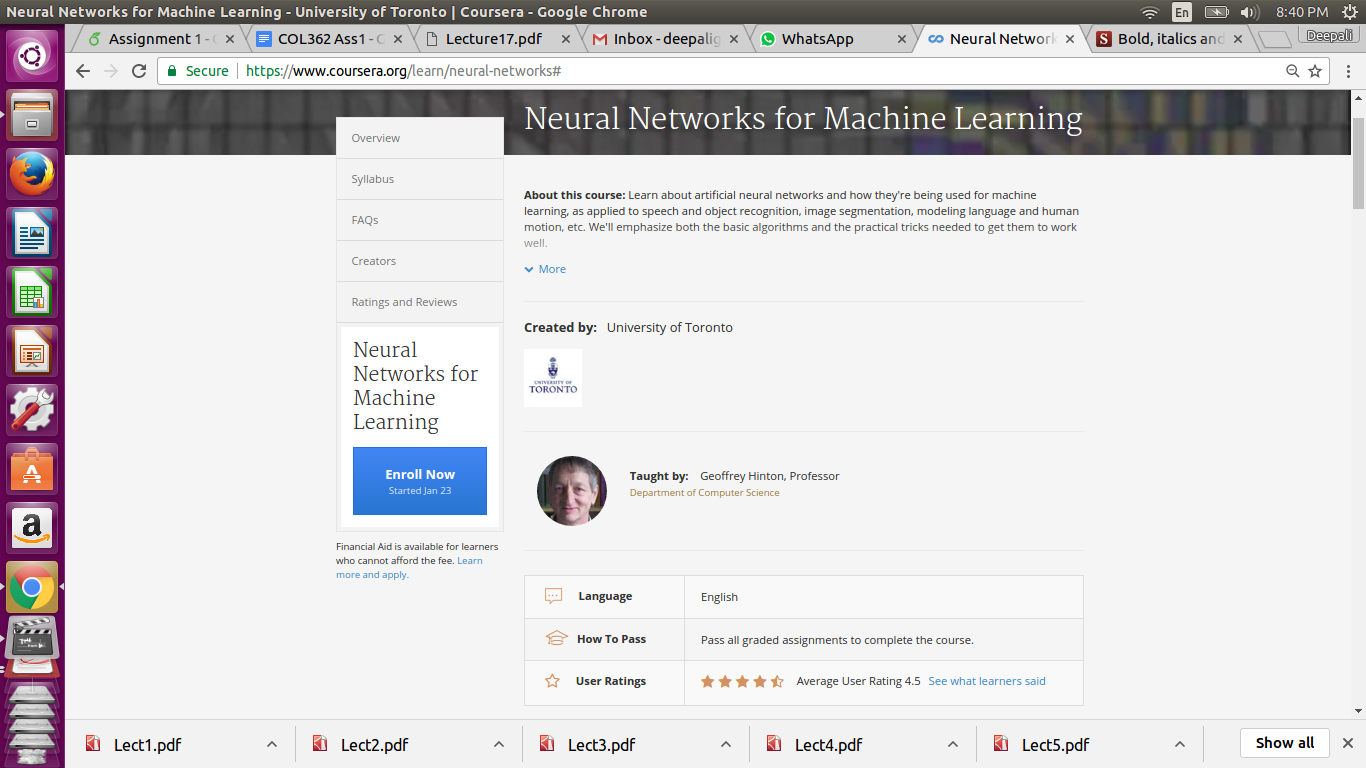
\includegraphics[width=18cm]{snap1.png}{\\Course Introduction Page}
\end{center}
\begin{center}
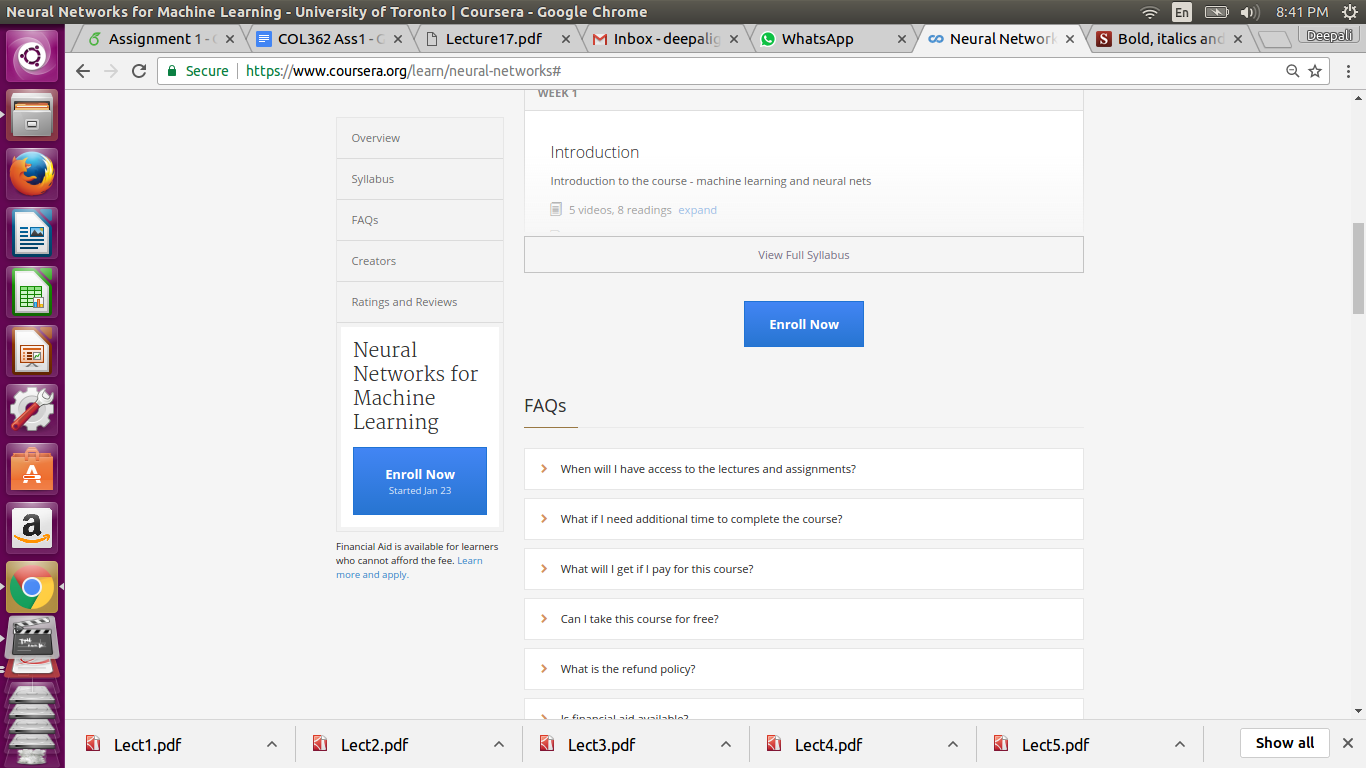
\includegraphics[width=18cm]{snap2.png}{\\Course Introduction Page}
\end{center}
\begin{center}
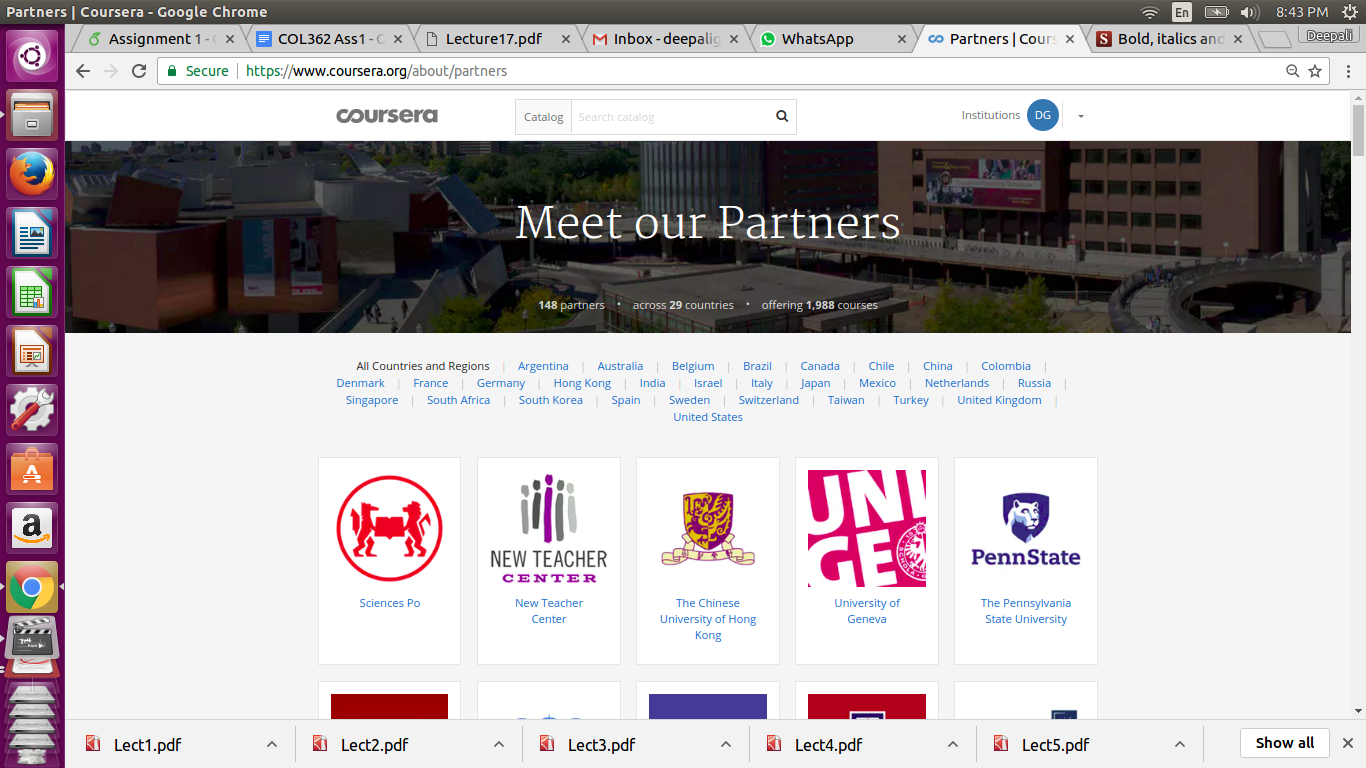
\includegraphics[width=18cm]{snap4.png}{\\Universities Page}
\end{center}
\begin{center}
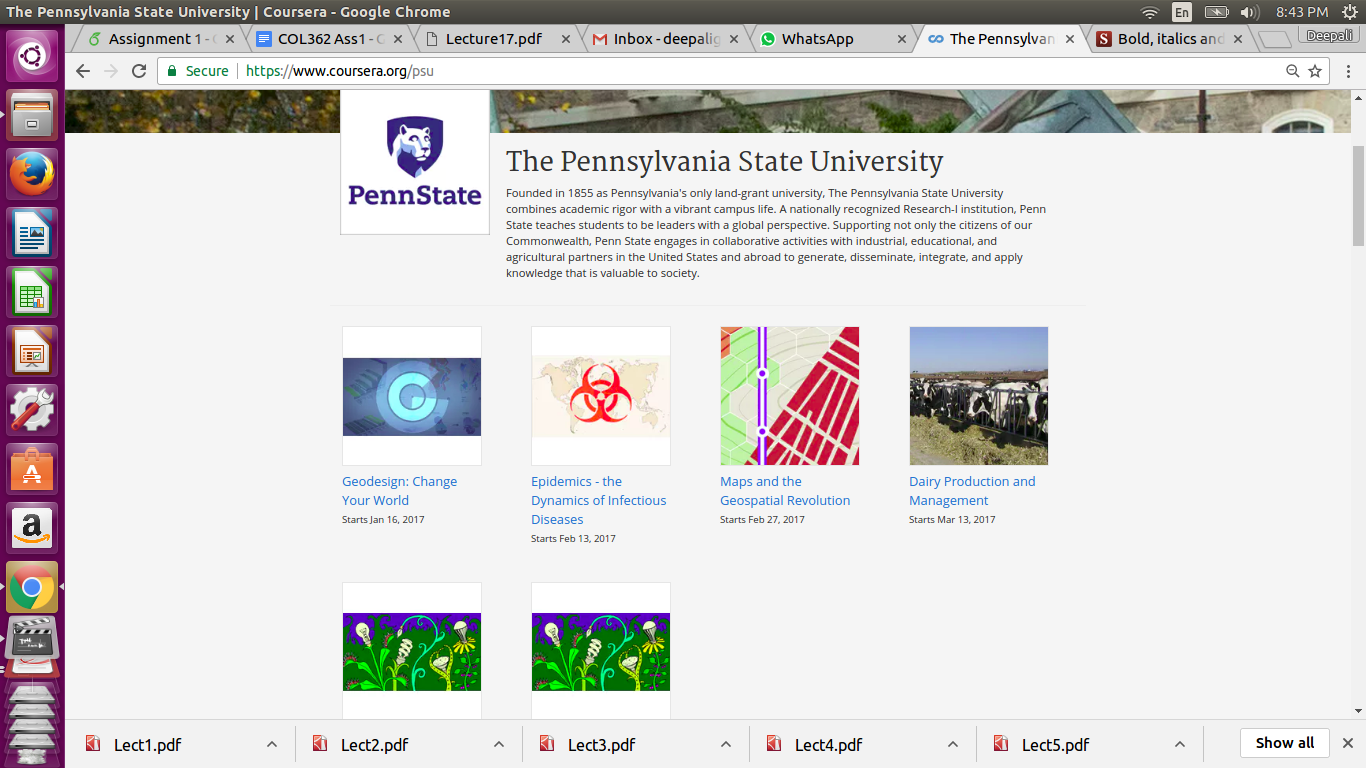
\includegraphics[width=18cm]{snap5.png}{\\University Details Page}
\end{center}
\begin{center}
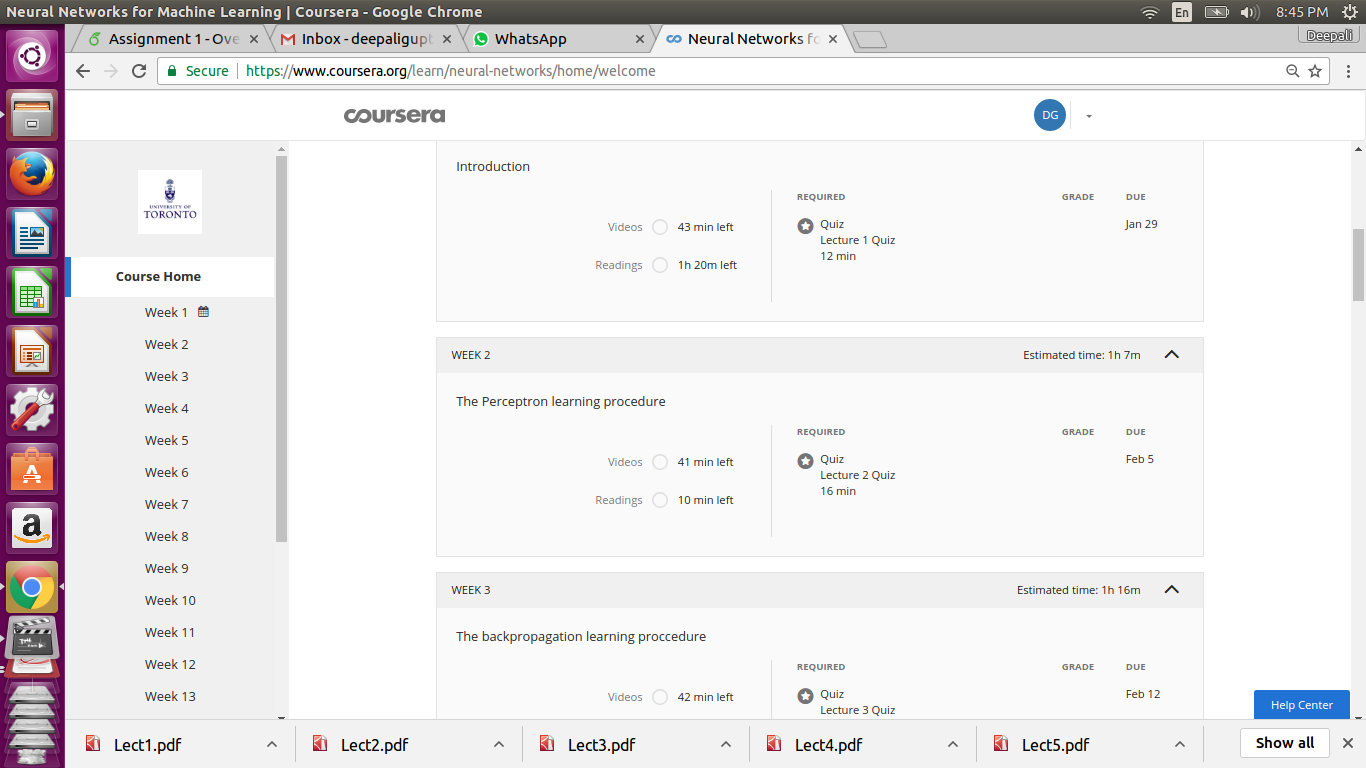
\includegraphics[width=18cm]{snap6.png}{\\Course Details Page}
\end{center}
\begin{center}
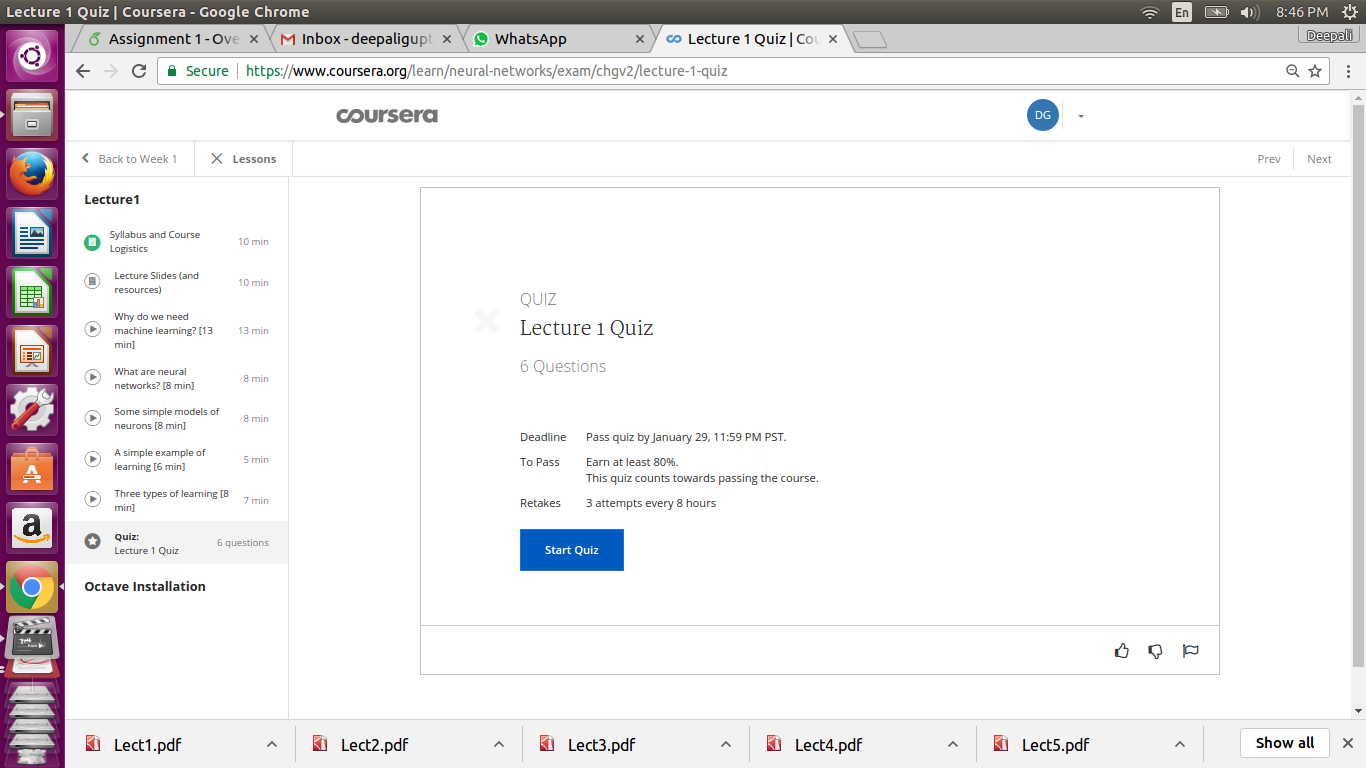
\includegraphics[width=18cm]{snap7.png}{\\Assignment Page}
\end{center}
\begin{center}
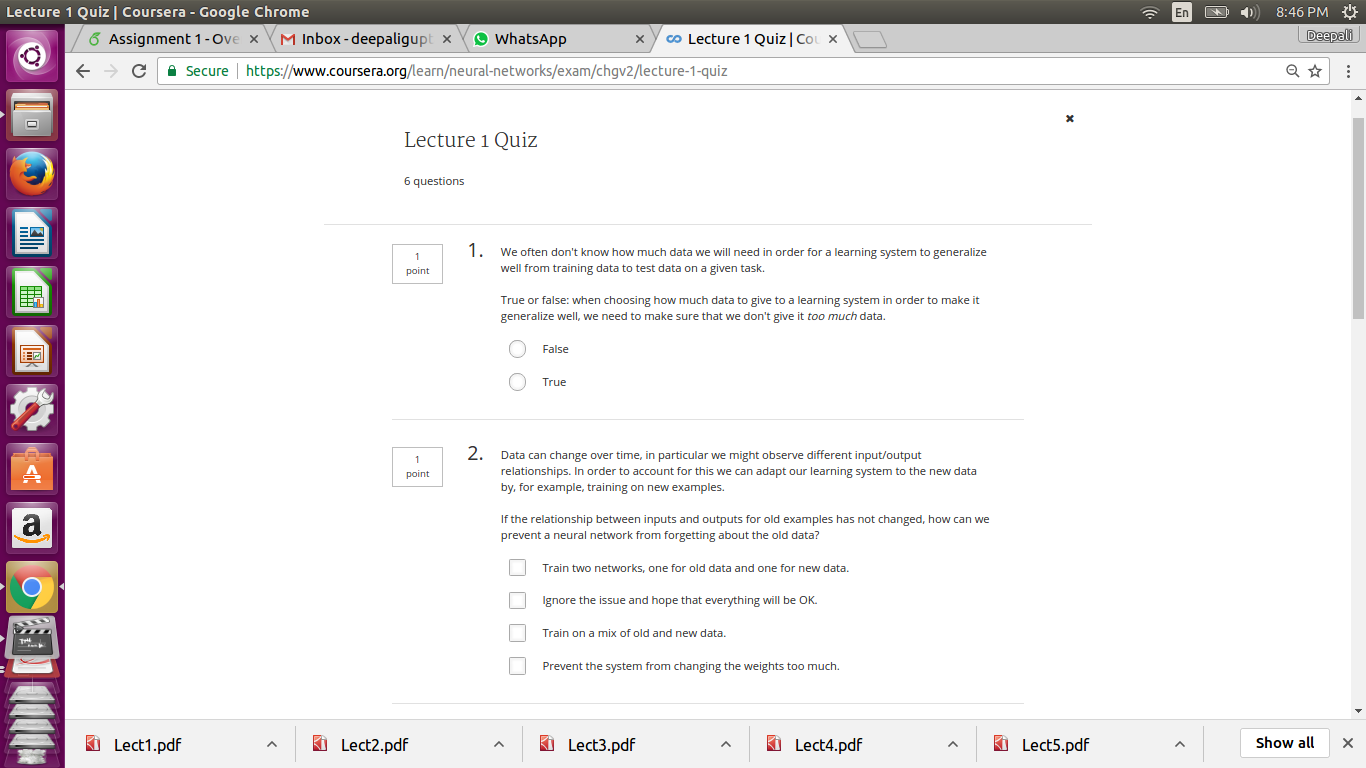
\includegraphics[width=18cm]{snap8.png}{\\Assignment Questions Page}
\end{center}
\begin{center}
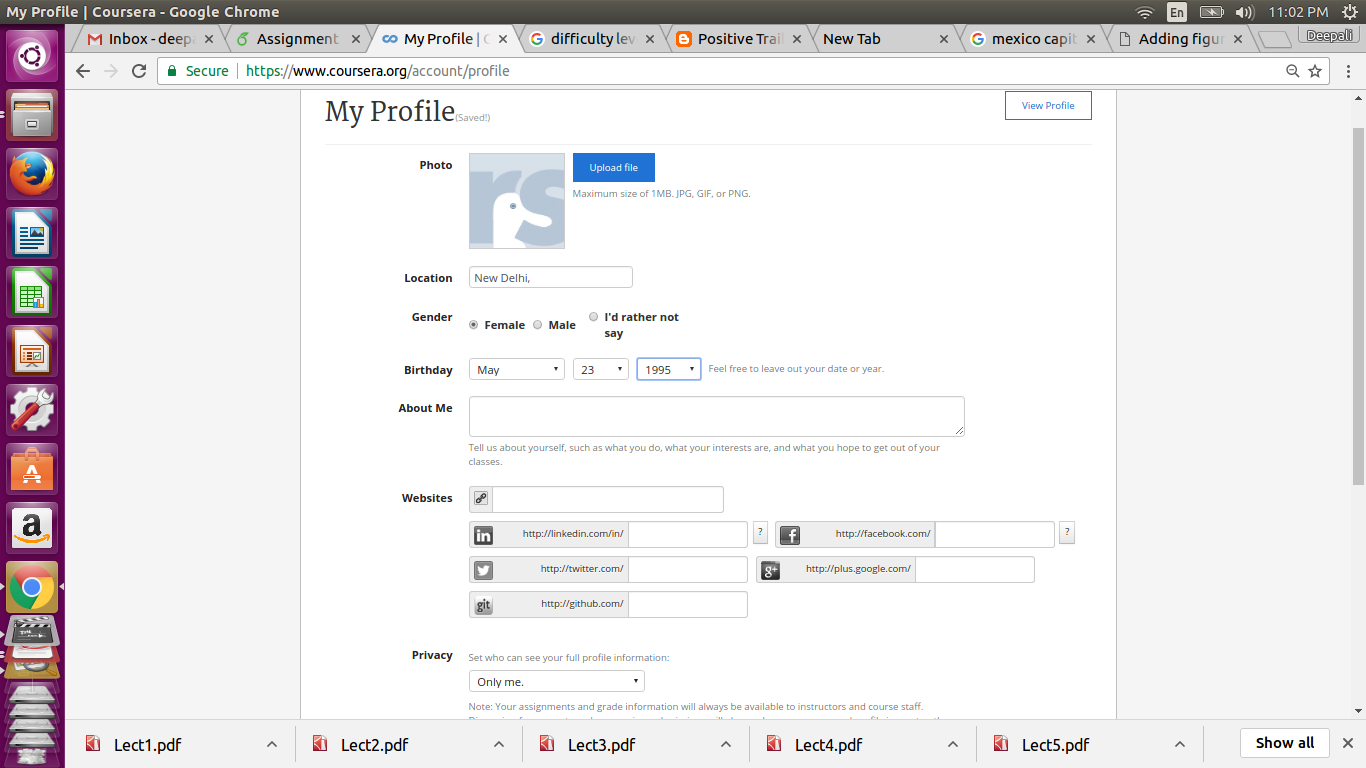
\includegraphics[width=18cm]{snap9.png}{\\User Profile Page}
\end{center}
\begin{center}
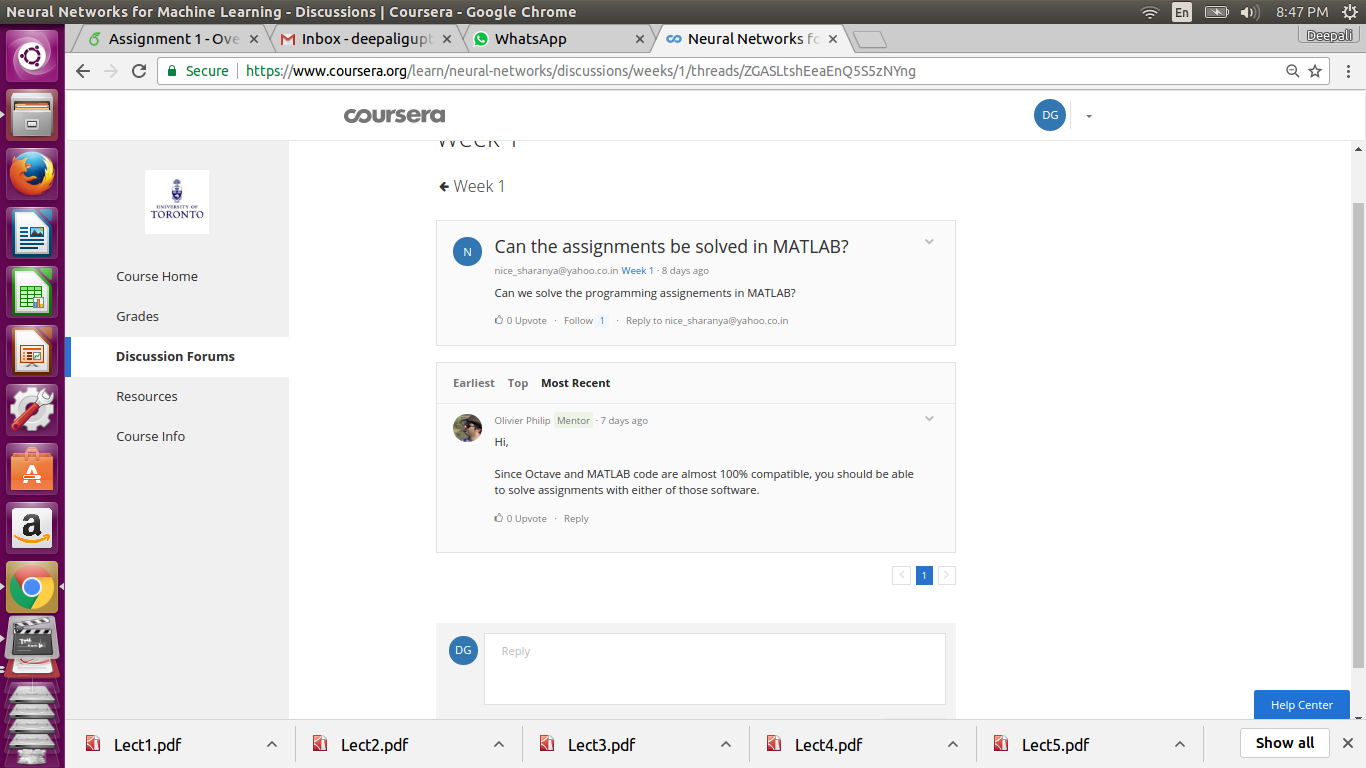
\includegraphics[width=18cm]{snap10.png}{\\Discussion Forum}
\end{center}

%%% Fill in your content here.
\subsection{List of various relationships}
\begin{table}[h!]
\centering
\caption{Relationships}
  \label{tab:table}
  \vspace{5mm}
  \begin{tabular}{|p{4cm}|p{10cm}|}
  \hline
  Type of relationship & Example\\
  \hline
  Weak Entity Set & (Assignment, Question), (Resource)\\
  \hline
  Non-Binary Relationship & (Course, User, Video)\\
  \hline
  Hierarchical Relationship & Instructor is a type of User\\
  \hline
  Type of relationship Constraint & All keys are unique and non null, User age must be in a valid range etc \\
  \hline
  Referential Constraint & ThreadID in comments refers to Thread, ForumID in thread refers to Forum, CourseID in thread refers to Course \\
  \hline
  \end{tabular}
\end{table}
%%% Fill in your content here.
\section{Answer 2}
Combining the attributes from tables: Course, User and Instructor, suppose we create a table with the following schema.\\
R(CourseID, Forum Topic, UserID, ThreadTitle, ThreadID, ForumID, ThreadViews, University Name,Contact Details)\\
For the purposes of example, we assume the following FD's in our data

\begin{itemize}
\item Contact Details $\rightarrow$ Name
\item(CourseID, Forum Topic) $\rightarrow$ ForumID
% \item Forum: (CourseID, Topic) $\rightarrow$ ForumID
\item (ForumID,UserID,Thread Title) $\rightarrow$ ThreadID
\item (ThreadID) $\rightarrow$ (Thread Title, Thread Views)
\item (ForumID) $\rightarrow$ (Forum Topic)
\item (ForumID,ThreadID) $\rightarrow$ (UserID)
\end{itemize}

We see that (CourseID, ForumTopic, UserID, ThreadTitle,Contact Details) forms a  key for this relation as its closure is the entire relation. Also, its minimal\\
\\
\textbf{Decomposition into 2NF}
In 2NF, no non prime attribute is dependent on proper subset of candidate key of the table. In the above relation, we see that the first three FD's violate this rule. So we decompose R into following relations :
\begin{itemize}
\item R1(\underline{Contact Details}, UniName)
\item R2(\underline{CourseID, Forum Topic}, Forum ID)
\item R3(\underline{ForumID,UserID, Thread Title}, Thread Views, ThreadID)
\item R4(\underline{CourseID, ForumTopic, UserID, Contact Details, Thread Title})
\end{itemize}
\textbf{Decomposition into 3 NF}
In 3 NF, no non prime attribute can depend can depend on another non prime attribute. We remove all the transitive dependencies.
\begin{itemize}
\item R2(a) (\underline{CourseID, ForumID})
\item R2(b) (\underline{ForumID}, ForumTopic)
\item R3(a) (\underline{ThreadID}, Thread Title, Thread Views)
\item R3(b) (\underline{ForumID, UserID, ThreadID})
\end{itemize}
\textbf{Decomposition into BCNF}
We see that the last FD is violating the BCNF criteria, so we modify relation 3(b).
\begin{itemize}
\item R3(b)(i) (\underline{ ForumID, ThreadID}, UserID)
\end{itemize}
%%% Fill in your content here.

\section{Answer 3}
\subsection{Schema}
\begin{table}[h!]
\centering
\caption{Dataset 1: Consumer Complaints}
  \label{tab:table}
  \vspace{5mm}
  \begin{tabular}{|p{4cm}|p{4cm}|}
  \hline
  Field Name & Data Type\\
  \hline
  ComplaintID & bigint\\
  \hline
  Product & varchar(40)\\
  \hline
  Issue & varchar(80)\\
  \hline
  Company & varchar(20)\\
  \hline
  State & char(2)\\
  \hline
  TimelyResponse & varchar(3)\\
  \hline
  \end{tabular}
\end{table}

\begin{table}[h!]
\centering
\caption{Dataset 2: Most Recent Cohorts Scorecard Elements}
  \label{tab:table5}
  \vspace{5mm}
  \begin{tabular}{|p{4cm}|p{4cm}|}
  \hline
  Field Name & Data Type\\
  \hline
  UnitID & bigint\\
  \hline
  INSTNM & varchar(40)\\
  \hline
  City & varchar(20)\\
  \hline
  Insturl & varchar(40)\\
  \hline
  Npcurl & varchar(100)\\
  \hline
  \end{tabular}
\end{table}

\begin{table}[h!]
\centering
\caption{Dataset 3: US Chronic Disease Indicators}
  \label{tab:table}
  \vspace{5mm}
  \begin{tabular}{|p{4cm}|p{4cm}|}
  \hline
  Field Name & Data Type\\
  \hline
  YearStart & char(4)\\
  \hline
  YearEnd & char(4)\\
  \hline
  LocationAbbr & char(2)\\
  \hline
  Topic & varchar(20)\\
  \hline
  Question & varchar(200)\\
  \hline
  Response & varchar(100)\\
  \hline
  \end{tabular}
\end{table}
%%% Fill in your content here.
\subsection{Various insert modes}
%%% Fill in your content here.
\subsubsection{Bulk Load}
Data was loaded from the csv files into the tables using the COPY command as follows:\linebreak
COPY consumer\_complaints FROM '~/Downloads/Consumer\_Complaints.csv' DELIMITER ',' csv;
%%% Fill in your content here.
\subsubsection{Insert statements}
A python script was written to load tuples from the csv file and place them into insert statements using psycopg2.
%%% Fill in your content here.
\subsubsection{JDBC}
A JDBC script was written to do a bulk insert.
%%% Fill in your content here.
\subsection{Statistics}
%%% Fill in your content here.
\underline{Machine Configuration}
\begin{itemize}
\item Processor : intel CORE i5
\item RAM : 8 GB
\item HDD : 1 TB
\item SSD : 125 GB
\item OS : Ubuntu 15.04
\item JDBC : Java 8
\end{itemize}

\begin{table}[h!]
\centering
\caption{Data Insertion Statistics}
  \label{tab:table}
  \vspace{5mm}
  \begin{tabular}{|p{2cm}|p{2cm}|p{1.5cm}|p{3.5cm}|p{3cm}|p{3cm}|}
  \hline
  Dataset No. & No. of tuples & Size(MB) & Bulk Load Time(ms) & Inserts Time(s) & JDBC Time(ms)\\
  \hline
  1 & 699224 & 59.5 & 3464.832 & 73 & 8649.273\\
  \hline
  2 & 53921 & 7 & 438.921 & 10 & 1357.538\\
  \hline
  3 & 237962 & 23 & 3837.433 & 35 & 7912.924 \\
  \hline
  \end{tabular}
\end{table}
\section{Answer 4}
%%% Fill in your content here.
A python script was written to duplicate the data in the previous datasets  by around 150 to 250 times.
\begin{table}[h!]
\centering
\caption{Data Insertion Statistics for Larger Datasets}
  \label{tab:table}
  \vspace{5mm}
   \begin{tabular}{|p{2cm}|p{2cm}|p{1.5cm}|p{3.5cm}|p{3cm}|p{3cm}|}
  \hline
  Dataset No. & No. of tuples & Size(GB) & Bulk Load Time(min) & Inserts Time(min) & JDBC Time(min)\\
  \hline
  1 & 99047410 & 8.3 & 20 & 76 & 26\\
  \hline
  2 & 39439360 & 5.1 & 8 & 48 & 12\\
  \hline
  3 & 63535854 & 6.5 & 14 & 59 & 19\\
  \hline
  \end{tabular}
\end{table}
\end{document}

\grid